% BrewLite A2 — Task 1.3. Fragment for inclusion into the A2 report.
% Requires in main preamble: \usepackage[utf8]{inputenc} (pdfLaTeX, if needed),
% \usepackage{longtable}, \usepackage{array}; Vietnamese UTF-8 engine/package per report template.
\section{Đặc tả Use Case trọng tâm --- Checkout}
\label{sec:a2-checkout}

\subsection{Mục tiêu và phạm vi}
Use Case \texttt{UC-A2-CHECKOUT-001} (mã đề xuất) mô tả quy trình Customer
xác nhận giỏ, tạo Order và thanh toán đến khi nhận được kết quả đáng tin cậy,
hoặc đến trạng thái chờ đối soát/hết hạn. Đặc tả liên kết UC-ORD-001 và
UC-PAY-001, sử dụng quy tắc trong Requirements v3.1 và API Contract v4.0.
Các khác biệt giữa đặc tả và implementation được ghi riêng bên dưới.

\subsection{Actor, Trigger và điều kiện}
\begin{description}
\item[Primary actor:] Customer đã đăng nhập.
\item[External supporting actor:] VNPay Sandbox (chỉ nhánh VNPay).
\item[Supporting components:] Frontend, Auth, Order, Pricing, Inventory, Coupon,
Payment, Finalization, Expiration/Reconciliation và Database.
\item[Trigger:] Customer nhấn Đặt hàng từ giỏ, sau đó chọn thanh toán.
\item[Precondition:] Customer có JWT hợp lệ để tạo Order và gửi được giỏ;
điều kiện tồn kho, coupon, Order active và expiry được xác minh trong flow.
\item[Success postcondition:] Order PAID, tối đa một Payment SUCCESS,
coupon CONSUMED/loyalty một lần và không trừ stock lần hai.
\item[Alternate postcondition:] Terminal FAILED trong TTL giữ tồn/coupon;
unknown giữ Payment PENDING; Order CANCELLED khi đủ điều kiện expiry thì
release tài nguyên đúng một lần.
\end{description}

\subsection{Main Success Flow}
\begin{enumerate}
\item Customer xác thực và gửi giỏ cùng coupon (nếu có) đến Order API.
\item Backend xác minh giỏ, Order active, giá/size/topping, tồn kho và coupon.
\item Backend tính tiền theo catalog, tạo Order PENDING cùng snapshot,
trừ/giữ tài nguyên nguyên tử; đặt expiresAt bằng createdAt cộng 15 phút.
\item Với totalVnd dương, Customer chọn VNPay; backend kiểm ownership,
TTL, idempotency và attempt trạng thái hiện tại rồi khởi tạo VNPay PENDING.
\item VNPay nhận thanh toán, gửi IPN; backend xác minh chữ ký, merchant,
TxnRef, amount, outcome và paid time. Return URL không đủ xác nhận SUCCESS.
\item Shared Finalization xác minh SUCCESS đúng hạn, Order chưa CANCELLED;
Payment SUCCESS, Order PAID, coupon CONSUMED, loyalty đúng một lần.
\item Frontend đọc Payment Status/Order History từ backend và hiển thị
kết quả; chỉ xóa giỏ khi đã xác nhận PAID.
\end{enumerate}

\subsection{Alternative và Exception Flows}
\begin{itemize}
\item Zero amount: dùng ZERO\_AMOUNT nội bộ, không gọi VNPay, pointsEarned=0.
\item Mock: chỉ khi được bật trong non-production và không có VNPay PENDING.
\item Kết quả FAILED đã xác minh: Order PAYMENT\_FAILED khi còn hạn; retry chỉ với attempt
mới sau xác nhận terminal failed.
\item TTL/Grace: không initiation từ expiresAt; VNPay PENDING có grace 5 phút
để đối soát thanh toán đã phát sinh đúng hạn. Hết grace còn unknown thì
Order CANCELLED/release, Payment có thể vẫn PENDING.
\item Wrong JWT/ownership: 401/404; invalid cart/stock/coupon: validation/409;
active Order: 409 PENDING\_ORDER\_EXISTS; idempotency mismatch: 409.
\item Invalid IPN, timeout, QueryDR unknown: không tự PAID/FAILED;
late financial SUCCESS sau CANCELLED lưu evidence, không hồi sinh Order.
\end{itemize}

\subsection{Traceability và giới hạn xác minh}
Chi tiết mọi nhánh, mã lỗi và traceability nằm trong tệp
\texttt{docs/requirements/}\allowbreak\texttt{A2\_T1.3\_Checkout\_}\allowbreak\texttt{Use\_Case\_Specification.md}.
Danh mục FR/NFR Checkout được liên kết với SRS và các endpoint được đối chiếu tĩnh với source. Các bảng dưới mô tả coverage yêu cầu và hiện thực, không đồng nghĩa kiểm thử runtime đã PASS.


% R-01 — Include editable original from docs/requirements/diagrams/checkout-use-case.drawio.
% Place this fragment in docs/report/sections/checkout-use-case.tex;
% place the companion PDF in docs/report/assets/checkout-use-case.pdf.
% Main report preamble must load graphicx: \usepackage{graphicx}.
\subsection{Use Case Diagram Checkout}
\begin{figure}[htbp]
\centering
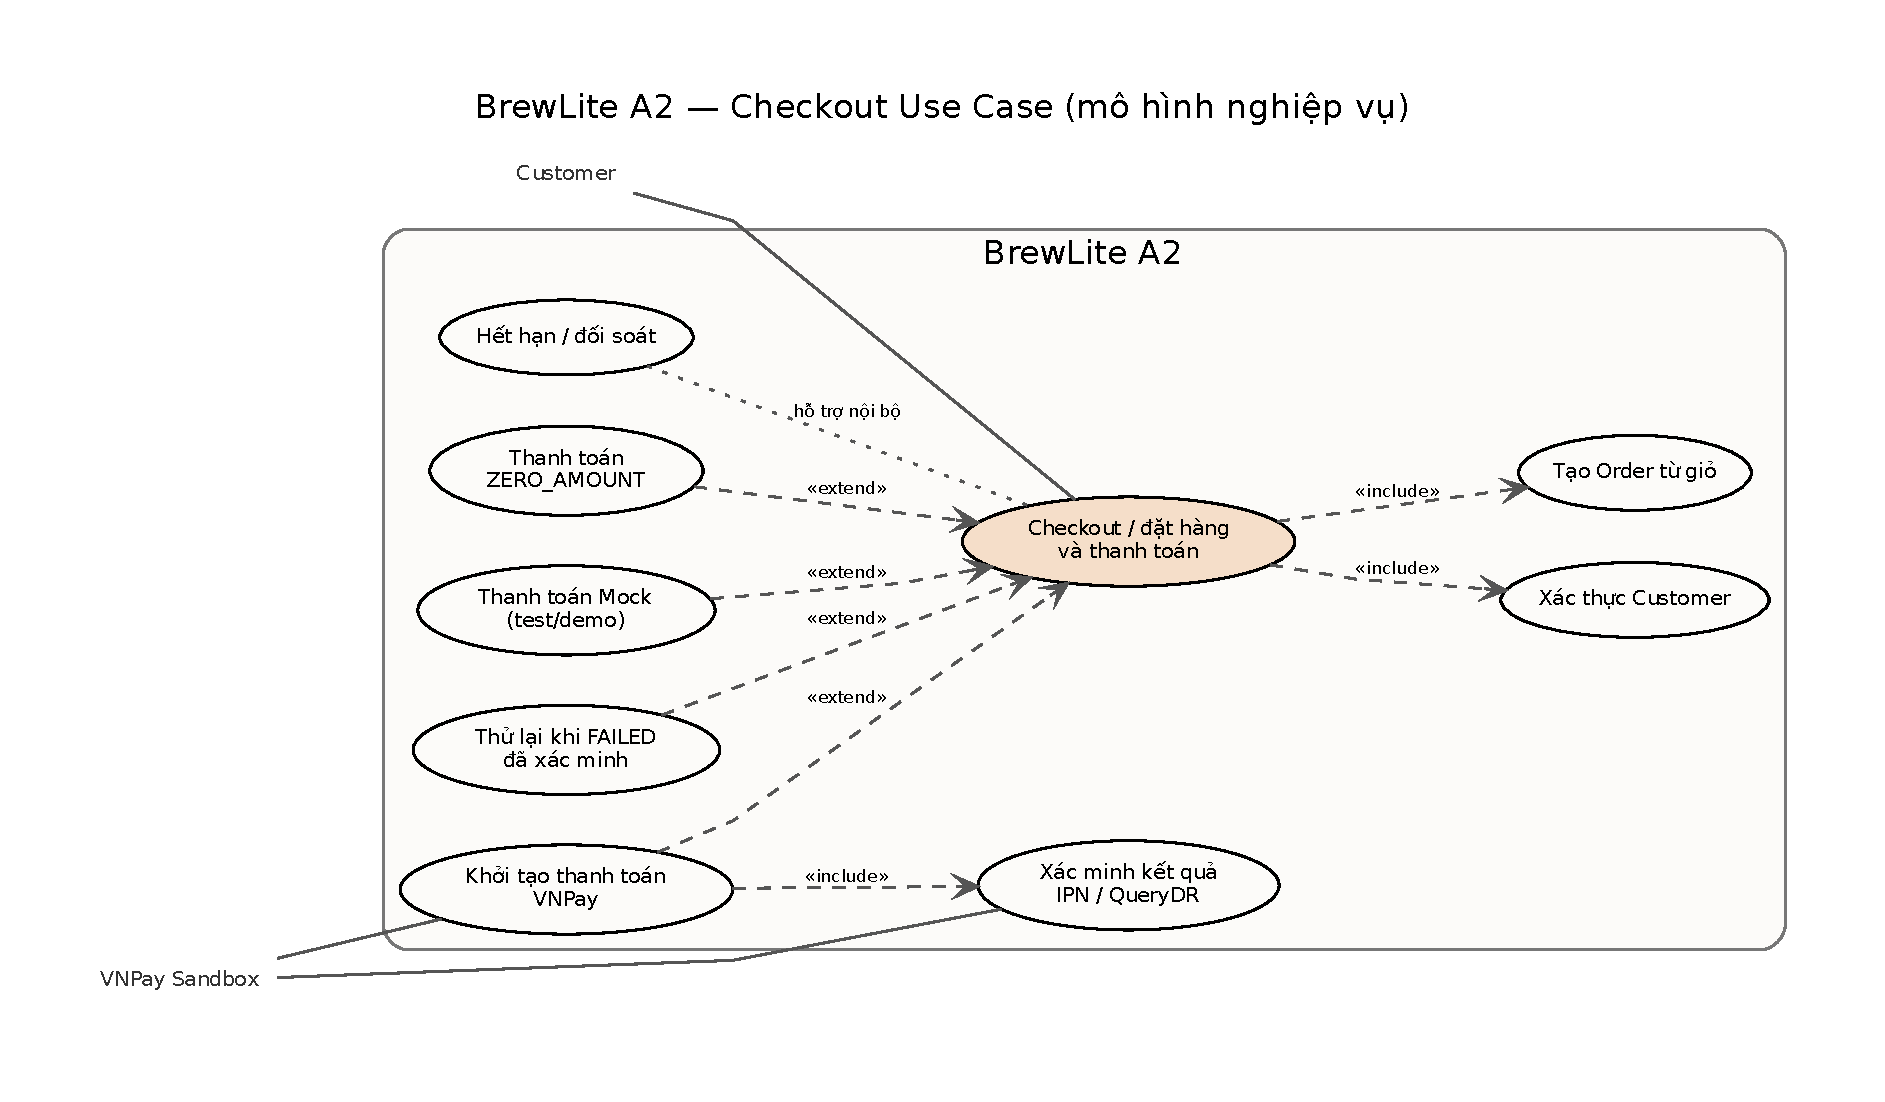
\includegraphics[width=\linewidth]{docs/report/assets/checkout-use-case.pdf}
\caption[Use Case Diagram Checkout]{Use Case Diagram Checkout --- Customer và VNPay Sandbox là actor ngoài; các service nội bộ không phải UML actor.}\label{tab:auto-checkout-use-case-1}
\label{fig:a2-checkout-use-case}
\end{figure}

\subsection{Liên kết yêu cầu Checkout}
Bảng liên kết Checkout với danh mục \path{docs/requirements/srs.md}; nguồn
được lưu trong đặc tả SRS và ma trận truy vết.
\begin{longtable}{|p{0.21\linewidth}|p{0.31\linewidth}|p{0.31\linewidth}|}
\caption{Checkout: mapping FR/NFR}\label{tab:auto-checkout-use-case-2}\\
\hline
\textbf{Nhóm Checkout} & \textbf{FR A2} & \textbf{NFR A2} \\ \hline
JWT / ownership & FR-03, FR-05--07 & NFR-01, 02, 05, 09 \\ \hline
Cart, giá, snapshot & FR-11, 17--20 & NFR-11, 12, 17, 27, 29 \\ \hline
Order active, tồn, coupon & FR-21, 24--28, 42, 46 & NFR-10, 13, 15, 18 \\ \hline
VNPay, retry, idempotency & FR-30--33, 36, 40 & NFR-15, 45, 46 \\ \hline
IPN / QueryDR / TTL & FR-25, 31, 37--39 & NFR-02, 16, 18, 43, 47, 48 \\ \hline
ZERO\_AMOUNT / Mock & FR-41 / FR-35 & NFR-10, 15, 48 / 49 \\ \hline
Status / Order History & FR-22, 34 & NFR-25--27 \\ \hline
Testing / logging / perf & FR-19, 30, 31 & NFR-20, 21, 33--36, 42 \\ \hline
\end{longtable}
FR-23 (hủy chủ động) và FR-43 (coupon preview) vẫn SHOULD/Deferred;
FR-29 inventory movement là SHOULD. Nhãn MUST* của NFR trong SRS
biểu thị phân loại ưu tiên đề xuất trong đặc tả. AC-A2 liên quan và mapping
đến từng bước nằm trong tài liệu Use Case chuẩn được dẫn ở trên.

\subsection{API và hiện thực Checkout}
Bảng đối chiếu API Contract v4.0 với inventory controller/service, app
baseline0e43bcb. Đây là kiểm tra source, không là nghiệm thu runtime hoặc
VNPay Sandbox E2E.
\begin{longtable}{|p{0.34\linewidth}|p{0.24\linewidth}|p{0.25\linewidth}|}
\caption{Checkout: API và implementation inventory}\label{tab:auto-checkout-use-case-3}\\
\hline
\textbf{Contract route} & \textbf{Kết quả} & \textbf{Source} \\ \hline
\texttt{POST /orders} & Có route & \texttt{orders.controller.ts} \\ \hline
\texttt{POST /payments/vnpay/initiate} & Có route & \texttt{payments.controller.ts} \\ \hline
\texttt{GET /payments/vnpay/ipn} & Có route & \texttt{vnpay-ipn.controller.ts} \\ \hline
\texttt{GET /payments/:paymentId/status} & Chưa có route & \texttt{payments.controller.ts} \\ \hline
\texttt{POST /payments/zero-amount} & Có route & \texttt{zero-amount-}\newline\texttt{payment.controller.ts} \\ \hline
\texttt{POST /payments} (Mock) & Có route & \texttt{payments.controller.ts} \\ \hline
\texttt{GET /orders/me} & Có route & \texttt{orders.controller.ts} \\ \hline
Internal QueryDR & Có service & \texttt{vnpay-querydr.service.ts} \\ \hline
\end{longtable}
Đường dẫn đầy đủ đến source/test và scope kiểm chứng được ghi ở bảng
inventory trong tài liệu Use Case chuẩn. Route Payment Status còn thiếu trong
backend; helper frontend tham chiếu route, còn UI hiện polling GET /orders/me.
Quyết định khép gap cần được xử lý theo phạm vi được duyệt. Source presence
không chứng minh behavior, integration tests hoặc Sandbox E2E đã PASS.

\subsection{Phân biệt trạng thái đối soát}
\texttt{REQUIRES\_REVIEW} là thông tin \emph{reconciliation} hoặc
\emph{resolution} cho UI; không phải trạng thái mới của Order hay
\texttt{Payment.status}. Trong tình huống sau Grace, Order có thể
\texttt{CANCELLED} còn Payment vẫn \texttt{PENDING}, đồng thời
\texttt{reconciliationState=REQUIRES\_REVIEW} khi hết horizon.
Không chuyển Payment thành FAILED chỉ vì kết quả chưa xác định.
